%!TEX program = lualatex
\documentclass[aspectratio=169,10pt]{beamer}

%%% ─── FONTS ─────────────────────────────────────────────────────────────────
\usepackage{fontspec}
\setsansfont{Carlito}
\setmainfont{Carlito}
\setmonofont{Carlito}
\usefonttheme{professionalfonts}

%%% ─── COLOURS ───────────────────────────────────────────────────────────────
\usepackage{xcolor}
\definecolor{navy}{RGB}{12,35,68}
\definecolor{navymid}{RGB}{38,76,140}
\definecolor{ice}{RGB}{228,238,252}
\definecolor{coal}{RGB}{45,45,45}
\definecolor{steel}{RGB}{148,158,172}
\definecolor{amber}{RGB}{205,90,10}

%%% ─── GRAPHICS / CHARTS ─────────────────────────────────────────────────────
\usepackage{tikz}
\usetikzlibrary{arrows.meta,positioning,calc,fit,backgrounds,shapes.geometric}
\usepackage{pgfplots}
\pgfplotsset{compat=1.18}

%%% ─── OTHER ─────────────────────────────────────────────────────────────────
\usepackage{booktabs}
\usepackage{array}
\usepackage{colortbl}
\usepackage{microtype}

%%% ─── BEAMER THEME ──────────────────────────────────────────────────────────
\usetheme{default}
\setbeamertemplate{navigation symbols}{}
\setbeamercolor{background canvas}{bg=white}

%% Frame title
\setbeamercolor{frametitle}{fg=navy,bg=white}
\setbeamerfont{frametitle}{size=\normalsize,series=\bfseries}
\setbeamertemplate{frametitle}{%
  \nointerlineskip
  \begin{beamercolorbox}[wd=\paperwidth,ht=2.0em,dp=0.4em,leftskip=0.6cm]{frametitle}%
    \vfill\usebeamerfont{frametitle}\insertframetitle\vfill
  \end{beamercolorbox}%
  \nointerlineskip
  {\color{navy}\hrule height 1.2pt}%
}

%% Footer
\setbeamertemplate{footline}{%
  {\color{steel!40}\hrule height 0.3pt}%
  \begin{beamercolorbox}[wd=\paperwidth,ht=1.6em,dp=0.4em,
      leftskip=0.6cm,rightskip=0.6cm]{footline}%
    {\tiny\color{steel}Understanding the Global Macro Landscape%
     \hfill\color{navy}\footnotesize\textbf{\insertframenumber}}%
  \end{beamercolorbox}%
}

%% Bullets
\setbeamertemplate{itemize item}{\color{navy}\small\textbullet}
\setbeamertemplate{itemize subitem}{\color{navymid}\small$\circ$}
\setbeamercolor{item}{fg=navy}
\setbeamerfont{itemize/enumerate body}{size=\small}
\setbeamerfont{itemize/enumerate subbody}{size=\footnotesize}

%% Blocks
\setbeamercolor{block title}{bg=navy,fg=white}
\setbeamercolor{block body}{bg=ice,fg=coal}
\setbeamerfont{block title}{size=\small,series=\bfseries}
\setbeamerfont{block body}{size=\footnotesize}

%%% ─── PGFPLOTS: ECONOMIST STYLE ─────────────────────────────────────────────
\pgfplotsset{
  %% Base: line charts, area charts, vertical bars
  econ/.style={
    width=\linewidth, height=3.5cm,
    axis line style={draw=steel!50, thin},
    axis x line*=bottom,
    axis y line=none,
    xmajorgrids=false,
    ymajorgrids=true,
    grid style={color=steel!25, thin},
    tick style={draw=none},
    every axis label/.style={font=\tiny, color=coal},
    every tick label/.style={font=\tiny, color=coal},
    title style={font=\scriptsize\bfseries\color{navy},
                 anchor=west, at={(axis description cs:0,1.13)}},
    legend style={draw=none,fill=none,font=\tiny},
    enlarge x limits=0.04,
    clip=false,
  },
  %% Horizontal bar charts
  econh/.style={
    width=\linewidth, height=3.5cm,
    xbar, bar width=7pt,
    axis line style={draw=steel!50, thin},
    axis y line=left,
    axis x line*=bottom,
    xmajorgrids=true,
    ymajorgrids=false,
    grid style={color=steel!25, thin},
    tick style={draw=none},
    every axis label/.style={font=\tiny, color=coal},
    every tick label/.style={font=\tiny, color=coal},
    title style={font=\scriptsize\bfseries\color{navy},
                 anchor=west, at={(axis description cs:0,1.13)}},
    enlarge y limits=0.25,
    clip=false,
  },
}

%%% ─── HELPERS ───────────────────────────────────────────────────────────────
\newcommand{\src}[1]{{\vspace{1pt}\par\raggedright\tiny\color{steel}\itshape #1}}
%% Short navy rule before chart/section titles (Economist signature)
\newcommand{\er}{{\textcolor{navy}{\rule{16pt}{2.5pt}}}\enspace}

%%% ═══════════════════════════════════════════════════════════════════════════
\begin{document}

%%% ─── TITLE SLIDE ────────────────────────────────────────────────────────────
\begin{frame}[plain]
\begin{tikzpicture}[remember picture,overlay]
  \fill[navy] (current page.south west) rectangle (current page.north east);
  %% Subtle horizontal stripe
  \fill[white,opacity=0.06]
    ([yshift=-0.56\paperheight]current page.north west)
    rectangle
    ([yshift=-0.59\paperheight]current page.north east);
  %% Content block
  \node[anchor=west, text width=0.86\paperwidth, align=left]
    at ([xshift=0.07\paperwidth]current page.west){%
    {\color{amber}\rule{24pt}{3pt}}\\[10pt]
    {\color{white}\fontsize{22}{28}\selectfont\bfseries
      Understanding the\\[4pt]Global Macro Landscape}\\[10pt]
    {\color{ice!85}\large From Headline Noise to Durable Capital Flows}\\[20pt]
    {\color{steel}\small
      Global Macro\ ·\ March 2026}\\[4pt]
    {\color{steel!60}\footnotesize
      For Educational Use Only}%
  };
\end{tikzpicture}
\end{frame}

%%% ═══════════════════════════════════════════════════════════════════════════
%%% EXECUTIVE SUMMARY
%%% ═══════════════════════════════════════════════════════════════════════════
\begin{frame}{The Three Things to Remember}
\begin{columns}[T,totalwidth=\textwidth]

\begin{column}{0.315\textwidth}
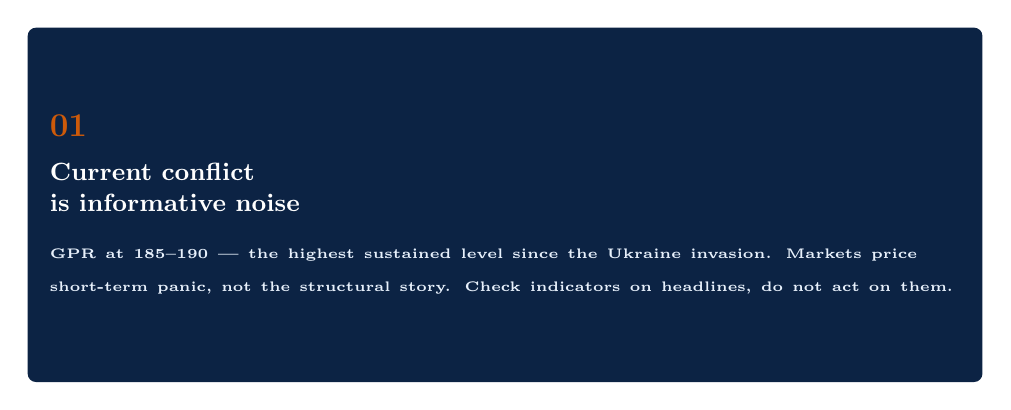
\begin{tikzpicture}
\node[fill=navy,text=white,rounded corners=3pt,
      text width={\dimexpr\linewidth-16pt\relax},inner sep=8pt,
      minimum height=4.5cm,align=left]{%
  {\color{amber}\large\bfseries 01}\\[5pt]
  \small\bfseries Current conflict\\ is informative noise\\[5pt]
  \tiny\color{ice!85}
  GPR at 185–190 — the highest sustained level since the Ukraine
  invasion. Markets price short-term panic, not the structural story.
  Check indicators on headlines, do not act on them.};
\end{tikzpicture}
\end{column}

\begin{column}{0.315\textwidth}
\begin{tikzpicture}
\node[fill=navy,text=white,rounded corners=3pt,
      text width={\dimexpr\linewidth-16pt\relax},inner sep=8pt,
      minimum height=4.5cm,align=left]{%
  {\color{amber}\large\bfseries 02}\\[5pt]
  \small\bfseries Watch events,\\ not news feeds\\[5pt]
  \tiny\color{ice!85}
  Capital deploys after: offtake agreement · project-finance close ·
  construction start · budget law.
  Everything else is noise to filter out.};
\end{tikzpicture}
\end{column}

\begin{column}{0.315\textwidth}
\begin{tikzpicture}
\node[fill=navy,text=white,rounded corners=3pt,
      text width={\dimexpr\linewidth-16pt\relax},inner sep=8pt,
      minimum height=4.5cm,align=left]{%
  {\color{amber}\large\bfseries 03}\\[5pt]
  \small\bfseries Three themes already attracting capital\\[5pt]
  \tiny\color{ice!85}
  Critical minerals + corridors · Defense procurement ·
  Low-carbon power. All three have confirmed commitment events and
  real capital flows as of March 2026.};
\end{tikzpicture}
\end{column}

\begin{column}{0.055\textwidth}
\end{column}
\end{columns}

\vspace{5pt}
%% Live numbers bar

\begin{tikzpicture}
\node[fill=ice,rounded corners=2pt,inner sep=5pt,
      text width={\dimexpr\textwidth-10pt\relax},align=center]{%
  \setlength{\tabcolsep}{6pt}
  \renewcommand{\arraystretch}{1.1}
  \begin{tabular}{@{}ccccc@{}}
    {\tiny\color{steel}Copper (LME)} &
    {\tiny\color{steel}GPR Index} &
    {\tiny\color{steel}DXY} &
    {\tiny\color{steel}WCI freight} &
    {\tiny\color{steel}Lobito committed} \\
    {\small\bfseries\color{navy}\$13{,}230/t} &
    {\small\bfseries\color{navy}185–190} &
    {\small\bfseries\color{navy}99.2} &
    {\small\bfseries\color{navy}\$1{,}899} &
    {\small\bfseries\color{navy}\$6\,bn+} \\
  \end{tabular}
  {\par\vspace{1pt}\tiny\color{steel}\itshape As of March 3, 2026 — sources cited per slide}};
\end{tikzpicture}
\end{frame}

%%% ═══════════════════════════════════════════════════════════════════════════
%%% 01 · CURRENT CONTEXT
%%% ═══════════════════════════════════════════════════════════════════════════
\begin{frame}{01 · Current Context}
\begin{columns}[T,totalwidth=\textwidth]

%% LEFT — quadrant positioning chart
\begin{column}{0.45\textwidth}
\vspace{2pt}
{\scriptsize\bfseries\color{navy}\er Where are we now?}\\[4pt]
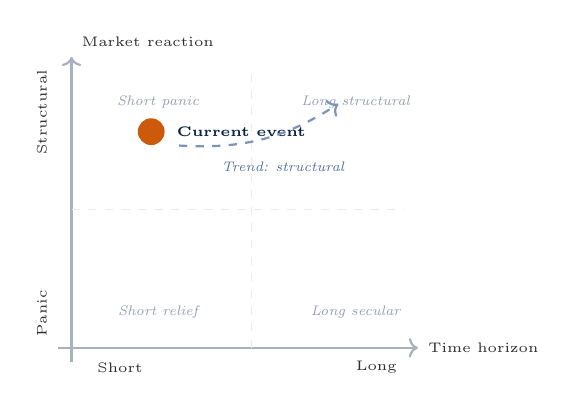
\begin{tikzpicture}[scale=0.88]
  \draw[->,steel!80,thick] (-0.2,0) -- (5.0,0)
    node[right,coal,font=\tiny]{Time horizon};
  \draw[->,steel!80,thick] (0,-0.2) -- (0,4.2)
    node[above right,coal,font=\tiny]{Market reaction};
  \node[font=\tiny,coal] at (0.7,-0.28)  {Short};
  \node[font=\tiny,coal] at (4.4,-0.28)  {Long};
  \node[font=\tiny,coal,rotate=90,anchor=south] at (-0.22,0.5)  {Panic};
  \node[font=\tiny,coal,rotate=90,anchor=south] at (-0.22,3.4) {Structural};
  \draw[steel!20,thin,dashed] (2.6,0)   -- (2.6,4.0);
  \draw[steel!20,thin,dashed] (0,2.0)   -- (4.8,2.0);
  \node[font=\tiny\itshape,steel] at (1.25,0.52) {Short relief};
  \node[font=\tiny\itshape,steel] at (4.10,0.52) {Long secular};
  \node[font=\tiny\itshape,steel] at (1.25,3.55) {Short panic};
  \node[font=\tiny\itshape,steel] at (4.10,3.55) {Long structural};
  %% current event
  \fill[amber] (1.15,3.12) circle (5.5pt);
  \node[font=\tiny\bfseries,navy,anchor=west] at (1.38,3.12)
    {Current event};
  %% trajectory
  \draw[->,navymid!60,thick,dashed]
    (1.55,2.92) to[bend right=18] (3.85,3.52);
  \node[font=\tiny\itshape,navymid!80] at (3.05,2.62)
    {\textit{Trend: structural}};
\end{tikzpicture}
{\tiny\color{steel}\itshape
  Headlines are signals to check indicators, not triggers to act immediately.}
\end{column}

%% RIGHT — GPR index line chart
\begin{column}{0.53\textwidth}
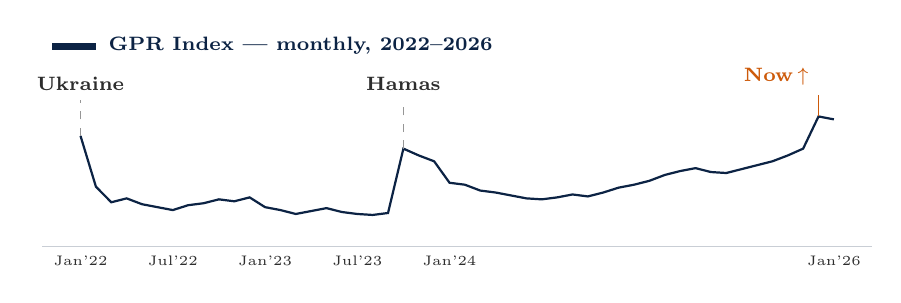
\begin{tikzpicture}
\begin{axis}[
  econ, height=3.65cm,
  title={\er GPR Index — monthly, 2022–2026},
  ytick={60,100,140,180},
  ymin=55, ymax=222,
  xtick={1,7,13,19,25,50},
  xticklabels={Jan'22,Jul'22,Jan'23,Jul'23,Jan'24,Jan'26},
  xmin=0.5, xmax=50.5,
]
%% Monthly data Jan 2022 – Feb 2026 (sequential month index 1..50)
%% Sources: Caldara & Iacoviello; Mar 2022 peak confirmed ~168 at Ukraine invasion;
%% Oct 2023 spike confirmed ~3× start-of-month (~155) at Hamas attack;
%% Early 2026 elevated ~185+ (US tariff shock + Ukraine ceasefire uncertainty)
\addplot[navy,thick,mark=none] coordinates {
  (1,168)(2,116)(3,100)(4,104)  % Jan–Apr 2022
  (5, 98)(6, 95)(7, 92)(8, 97)  % May–Aug 2022
  (9, 99)(10,103)(11,101)(12,105)% Sep–Dec 2022
  (13,95)(14,92)(15,88)(16,91)  % Jan–Apr 2023
  (17,94)(18,90)(19,88)(20,87)  % May–Aug 2023
  (21,89)(22,155)(23,148)(24,142)% Sep–Dec 2023 (Oct Hamas spike)
  (25,120)(26,118)(27,112)(28,110)% Jan–Apr 2024
  (29,107)(30,104)(31,103)(32,105)% May–Aug 2024
  (33,108)(34,106)(35,110)(36,115)% Sep–Dec 2024
  (37,118)(38,122)(39,128)(40,132)% Jan–Apr 2025
  (41,135)(42,131)(43,130)(44,134)% May–Aug 2025
  (45,138)(46,142)(47,148)(48,155)% Sep–Dec 2025
  (49,188)(50,185)               % Jan–Feb 2026 (tariff/Ukraine spike)
};
\draw[coal!50,thin,dashed]
  (axis cs:1,168) -- (axis cs:1,205)
  node[anchor=south,font=\scriptsize\bfseries,coal]{Ukraine};
\draw[coal!50,thin,dashed]
  (axis cs:22,155) -- (axis cs:22,205)
  node[anchor=south,font=\scriptsize\bfseries,coal]{Hamas};
\draw[amber,thin]
  (axis cs:49,188) -- (axis cs:49,210)
  node[anchor=south east,font=\scriptsize\bfseries,amber]{Now\,$\uparrow$};
\end{axis}
\end{tikzpicture}
\src{Caldara \& Iacoviello GPR Index (matteoiacoviello.com). Monthly. Mar\,2022 spike confirmed\,=\,168; Oct\,2023 spike\,$\approx$\,155; Jan\,2026\,$\approx$\,185–190.}
\end{column}

\end{columns}
\end{frame}

%%% ═══════════════════════════════════════════════════════════════════════════
%%% HISTORICAL PRECEDENTS
%%% ═══════════════════════════════════════════════════════════════════════════
\begin{frame}{Historical Precedents — Markets Recover After Geopolitical Shocks}
\begin{columns}[T,totalwidth=\textwidth]

\begin{column}{0.54\textwidth}
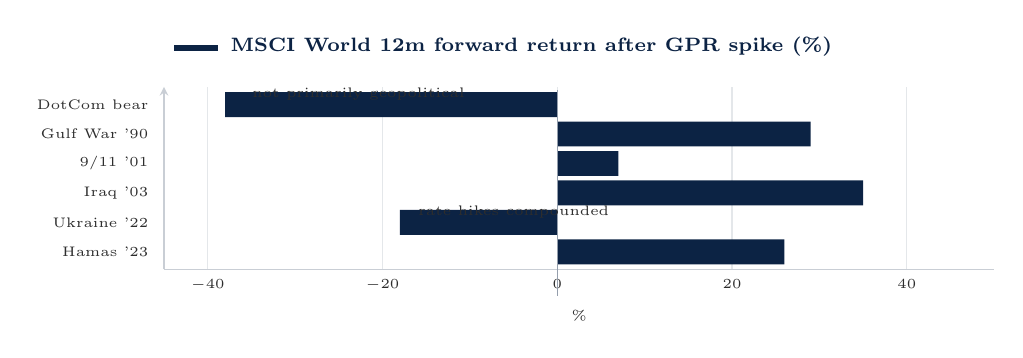
\begin{tikzpicture}
\begin{axis}[
  econh, height=3.9cm,
  title={\er MSCI World 12m forward return after GPR spike (\%)},
  xlabel={\%},
  ytick={1,2,3,4,5,6},
  yticklabels={Hamas '23,Ukraine '22,Iraq '03,9/11 '01,Gulf War '90,DotCom bear},
  y tick label style={font=\tiny,color=coal},
  xmin=-45, xmax=50,
  xtick={-40,-20,0,20,40},
  bar width=9pt,
  enlarge y limits=0.12,
]
%% 12-month forward returns (MSCI World) after each event
%% Sources: Bloomberg / MSCI. Gulf War: S&P +29% 12mo; 9/11 in existing bear market +7%;
%% Iraq War coincided with bear market bottom +35%; DotCom+9/11 combined bear -38%;
%% Ukraine 2022: MSCI World full year -18% (rate hikes compounded); Hamas +26% 12mo.
\addplot[fill=navy,draw=none] coordinates {
  (26,1)
  (-18,2)
  (35,3)
  (7,4)
  (29,5)
  (-38,6)
};
%% Zero line
\draw[steel,thin] (axis cs:0,-0.5) -- (axis cs:0,6.5);
%% Annotation on Ukraine
\node[font=\tiny,coal,anchor=west] at (axis cs:-17,2.35)
  {\tiny rate hikes compounded};
\node[font=\tiny,coal,anchor=west] at (axis cs:-36,6.35)
  {\tiny not primarily geopolitical};
\end{axis}
\end{tikzpicture}
\src{Bloomberg / MSCI World TR. 12-month returns from event date. Ukraine\,=\,calendar year 2022 (rate-hike compound effect). Educational — not forward guidance.}
\end{column}

\begin{column}{0.44\textwidth}
\vspace{4pt}
{\scriptsize\bfseries\color{navy}\er The pattern}\\[4pt]
{\footnotesize
\begin{itemize}\setlength\itemsep{2pt}
  \item Geopolitical shocks cause \textbf{short-term panic} — not structural damage to diversified portfolios
  \item Pure geopolitical events (Gulf War, Iraq War, Hamas) show \textbf{strong 12-month recoveries}
  \item Exceptions: shocks that \textbf{compound with financial crises} or rate-hike cycles
  %\item \textbf{Conclusion}: check indicators on headlines; deploy into conviction themes when commitment events confirm
\end{itemize}
}
\vspace{3pt}
\begin{block}{\small Rule of thumb}
{\footnotesize Investors who stayed diversified and systematic through all six events outperformed those who moved to cash.}
\end{block}
\end{column}

\end{columns}
\end{frame}

%%% ═══════════════════════════════════════════════════════════════════════════
%%% 02 · TRANSMISSION CHANNELS
%%% ═══════════════════════════════════════════════════════════════════════════
\begin{frame}{02 · Transmission Channels}
\begin{columns}[T,totalwidth=\textwidth]

\begin{column}{0.42\textwidth}
{\scriptsize\bfseries\color{navy}\er Conflict → asset re-pricing}\\[5pt]
\begin{tikzpicture}[
  nd/.style={rectangle,rounded corners=2pt,fill=navy,text=white,
             font=\tiny\bfseries,inner sep=5pt,
             text width=3.15cm,align=center,minimum height=0.70cm},
  ar/.style={->,navy!55,thick,shorten >=2pt,shorten <=2pt},
  node distance=0.50cm,
]
  \node[nd](A){Conflict / Escalation};
  \node[nd,below=of A](B){Shipping Chokepoints\\
    {\tiny\color{ice!80}Red Sea · Hormuz · Black Sea}};
  \node[nd,below=of B](C){Freight \& Insurance $\uparrow$\\
    {\tiny\color{ice!80}WCI: \$1{,}500\,$\to$\,\$5{,}901 (+293\%)}};
  \node[nd,below=of C](D){Energy \& Input Prices\\
    {\tiny\color{ice!80}Fuel surcharges · materials}};
  \node[nd,below=of D](E){Asset Re-pricing\\
    {\tiny\color{ice!80}Equities · spreads · FX}};
  \draw[ar](A)--(B);
  \draw[ar](B)--(C);
  \draw[ar](C)--(D);
  \draw[ar](D)--(E);
  \node[font=\tiny\itshape,coal,anchor=west,
        right=0.1cm of B,text width=1.9cm]
    {Alternative\\corridors:\\Cape route,\\Lobito};
\end{tikzpicture}
\end{column}

\begin{column}{0.56\textwidth}
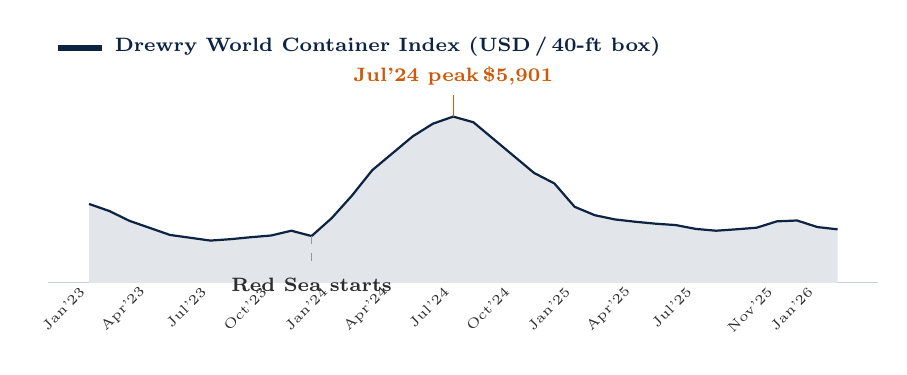
\begin{tikzpicture}
\begin{axis}[
  econ, height=4.05cm,
  title={\er Drewry World Container Index (USD\,/\,40-ft box)},
  ylabel={USD},
  ylabel style={at={(axis description cs:-0.05,0.5)},rotate=90},
  ytick={0,2000,4000,6000},
  ymin=0, ymax=6900,
  xtick={1,4,7,10,13,16,19,22,25,28,31,35,37},
  xticklabels={Jan'23,Apr'23,Jul'23,Oct'23,Jan'24,Apr'24,Jul'24,Oct'24,Jan'25,Apr'25,Jul'25,Nov'25,Jan'26},
  x tick label style={rotate=45,anchor=east,font=\tiny},
  xmin=0.5, xmax=38.5,
]
%% Weekly Drewry WCI, monthly approximation Jan 2023 – Feb 2026
%% Key anchors (confirmed data):
%%  Jan 2023 ~$2,800; Dec 2023: ~$1,661 (confirmed);
%%  Jul 2024 peak: ~$5,901–$5,937 (confirmed); Dec 2024 ~$3,529 (confirmed, YTD avg $3,949);
%%  Sep 2025: $1,913 (confirmed); Dec 2025: ~$2,182–$2,213 (confirmed); Feb 2026: $1,899 (confirmed)
\addplot[fill=navy!12,draw=none] coordinates {
  % 2023 (months 1-12): Red Sea rerouting begins Dec 2023
  (1,2800)(2,2550)(3,2200)(4,1950)(5,1700)(6,1600)
  (7,1500)(8,1550)(9,1620)(10,1680)(11,1850)(12,1661)
  % 2024 (months 13-24): massive surge on Red Sea crisis
  (13,2300)(14,3100)(15,4000)(16,4600)(17,5200)(18,5650)
  (19,5901)(20,5700)(21,5100)(22,4500)(23,3900)(24,3529)
  % 2025 (months 25-36): gradual normalisation, year-end tick up
  (25,2700)(26,2400)(27,2250)(28,2168)(29,2100)(30,2050)
  (31,1913)(32,1850)(33,1900)(34,1957)(35,2182)(36,2213)
  % 2026 Jan-Feb
  (37,1980)(38,1899)
} \closedcycle;
\addplot[navy,thick,mark=none] coordinates {
  (1,2800)(2,2550)(3,2200)(4,1950)(5,1700)(6,1600)
  (7,1500)(8,1550)(9,1620)(10,1680)(11,1850)(12,1661)
  (13,2300)(14,3100)(15,4000)(16,4600)(17,5200)(18,5650)
  (19,5901)(20,5700)(21,5100)(22,4500)(23,3900)(24,3529)
  (25,2700)(26,2400)(27,2250)(28,2168)(29,2100)(30,2050)
  (31,1913)(32,1850)(33,1900)(34,1957)(35,2182)(36,2213)
  (37,1980)(38,1899)
};
\draw[amber,thin]
  (axis cs:19,5901) -- (axis cs:19,6650)
  node[anchor=south,font=\scriptsize\bfseries,amber]{Jul'24 peak\,\$5{,}901};
\draw[coal!50,thin,dashed]
  (axis cs:12,1661) -- (axis cs:12,500)
  node[anchor=north,font=\scriptsize\bfseries,coal]{Red Sea starts};
\end{axis}
\end{tikzpicture}
\src{Drewry WCI (drewry.co.uk). Confirmed anchors: Jul\,2024\,=\,\$5{,}901; Dec\,2024\,=\,\$3{,}529; Sep\,2025\,=\,\$1{,}913; Feb\,2026\,=\,\$1{,}899.}
{\tiny\color{coal}Higher freight raises input costs (autos, electronics, apparel)
and widens spreads for EM USD borrowers.}
\end{column}

\end{columns}
\end{frame}

%%% ═══════════════════════════════════════════════════════════════════════════
%%% 03 · DURABLE RE-MAPPING
%%% ═══════════════════════════════════════════════════════════════════════════
\begin{frame}{03 · Durable Re-mapping of Capital}
{\small\color{coal}
  Conflict accelerates an ongoing geoeconomic shift.
  Five long-term themes attract committed capital.}
\vspace{8pt}

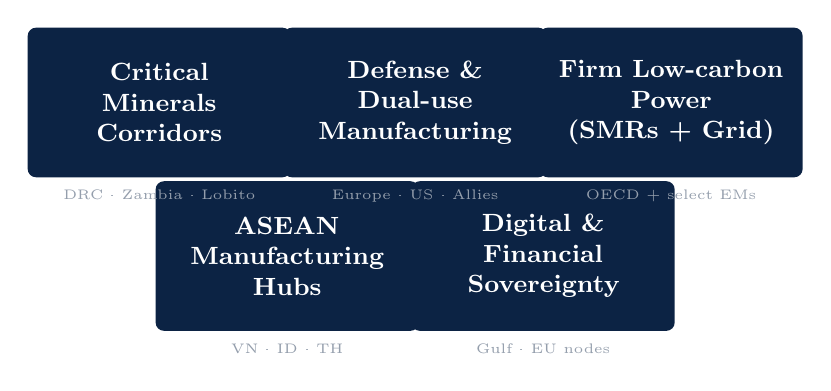
\begin{tikzpicture}[
  box/.style={rectangle,rounded corners=3pt,fill=navy,text=white,
              font=\small\bfseries,inner sep=7pt,
              text width=2.85cm,minimum height=1.9cm,align=center},
  sub/.style={font=\tiny,color=steel,align=center},
]
  \node[box](M) at (0,0)     {Critical\\Minerals\\Corridors};
  \node[box](D) at (3.25,0)  {Defense \&\\Dual-use\\Manufacturing};
  \node[box](E) at (6.5,0)   {Firm Low-carbon\\Power\\(SMRs + Grid)};
  \node[box](A) at (1.625,-1.95) {ASEAN\\Manufacturing\\Hubs};
  \node[box](S) at (4.875,-1.95) {Digital \&\\Financial\\Sovereignty};

  \node[sub,below=1pt of M] {DRC · Zambia · Lobito};
  \node[sub,below=1pt of D] {Europe · US · Allies};
  \node[sub,below=1pt of E] {OECD + select EMs};
  \node[sub,below=1pt of A] {VN · ID · TH};
  \node[sub,below=1pt of S] {Gulf · EU nodes};

\end{tikzpicture}
\end{frame}

%%% ═══════════════════════════════════════════════════════════════════════════
%%% 04 · WHO UNDERPERFORMS
%%% ═══════════════════════════════════════════════════════════════════════════
\begin{frame}{04 · Structural Headwinds — Who Likely Underperforms}
\begin{columns}[T,totalwidth=\textwidth]

\begin{column}{0.56\textwidth}
\renewcommand{\arraystretch}{1.38}
\setlength{\tabcolsep}{4pt}
\begin{tabular}{>{\small\bfseries}p{3.0cm}%
                >{\footnotesize}p{3.80cm}}
  \rowcolor{navy}
    \color{white}Sector & \color{white}Structural headwind \\
  \rowcolor{ice}
    Shipping hubs \& low-margin ports &
    Higher insurance and freight; rerouting risk \\
  Airlines \& tourism near conflict zones &
    Fuel/insurance surge + demand shock \\
  \rowcolor{ice}
    High-debt EMs with USD liabilities &
    Strong USD + tighter external funding \\
  Low-value manufacturing in risky jurisdictions &
    Friend-shoring away; sustained FDI outflows \\
\end{tabular}
\vspace{6pt}
{\footnotesize\color{coal}
  Structural headwinds, not temporary disruptions.\\
  Exposure may persist \textbf{3–7 years} as supply chains re-route.}
\end{column}

\begin{column}{0.42\textwidth}
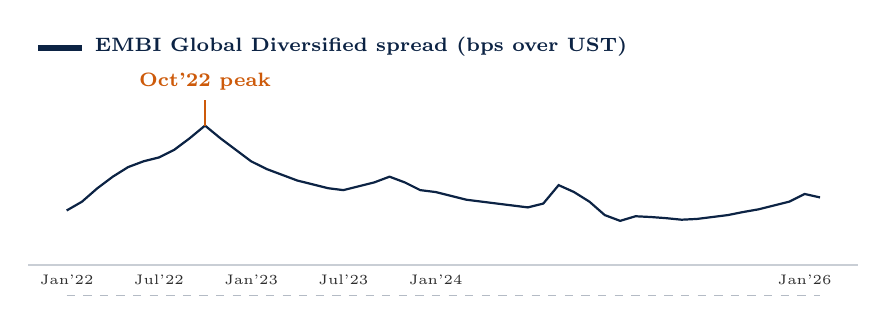
\begin{tikzpicture}
\begin{axis}[
  econ, height=3.85cm,
  title={\er EMBI Global Diversified spread (bps over UST)},
  ylabel={bps},
  ylabel style={at={(axis description cs:-0.05,0.5)},rotate=90},
  ytick={200,300,400,500,600},
  ymin=180, ymax=645,
  xtick={1,7,13,19,25,49},
  xticklabels={Jan'22,Jul'22,Jan'23,Jul'23,Jan'24,Jan'26},
  xmin=0.5, xmax=50.5,
]
%% Monthly EMBI GD spread Jan 2022 – Feb 2026 (sequential 1..50)
%% Key confirmed anchors:
%%  Oct 2022 end: ~543 bps (confirmed); Sep 2024: 388 bps (confirmed);
%%  Jan 2025: spreads ~86bps tighter y/y vs Jan 2024; Feb 2025: ~+12bps widening;
%%  Late 2024 / early 2025 spreads at "historical tights" ~280–310 bps
\addplot[navy,thick,mark=none] coordinates {
  % 2022 Jan–Dec: Russia invasion drives sharp widening to ~540 in Oct, then recovery
  (1,322)(2,345)(3,380)(4,410)(5,435)(6,450)
  (7,460)(8,480)(9,510)(10,543)(11,510)(12,480)
  % 2023 Jan–Dec: gradual compression
  (13,450)(14,430)(15,415)(16,400)(17,390)(18,380)
  (19,375)(20,385)(21,395)(22,410)(23,395)(24,375)
  % 2024 Jan–Dec: continued tightening; Sep confirmed 388, year-end ~310
  (25,370)(26,360)(27,350)(28,345)(29,340)(30,335)
  (31,330)(32,340)(33,388)(34,370)(35,345)(36,310)
  % 2025 Jan–Dec: historically tight; Feb +12bps; gradual widening H2
  (37,295)(38,307)(39,305)(40,302)(41,298)(42,300)
  (43,305)(44,310)(45,318)(46,325)(47,335)(48,345)
  % 2026 Jan–Feb
  (49,365)(50,356)
};
\draw[amber,thin]
  (axis cs:10,543) -- (axis cs:10,610)
  node[anchor=south,font=\scriptsize\bfseries,amber]{Oct'22 peak};
\draw[steel!70,thin,dashed]
  (axis cs:1,100) -- (axis cs:50,100);
\end{axis}
\end{tikzpicture}
\src{JPMorgan EMBI Global Diversified. Oct\,2022\,=\,543\,bps (confirmed); Sep\,2024\,=\,388\,bps (confirmed); year-end 2024\,$\approx$\,310\,bps (historically tight).}
\end{column}

\end{columns}
\end{frame}

%%% ═══════════════════════════════════════════════════════════════════════════
%%% 05 · WHO WINS
%%% ═══════════════════════════════════════════════════════════════════════════
\begin{frame}{05 · Long-term Winners — Sectors × Geographies}
\begin{columns}[T,totalwidth=\textwidth]

\begin{column}{0.53\textwidth}
\renewcommand{\arraystretch}{1.30}
\setlength{\tabcolsep}{3pt}
\begin{tabular}{>{\scriptsize\bfseries}p{2.42cm}%
                >{\scriptsize}p{1.65cm}%
                >{\scriptsize}p{2.42cm}}
  \rowcolor{navy}
    \color{white}Theme & \color{white}Where & \color{white}Why \\
  \rowcolor{ice}
    Critical minerals & DRC, Zambia, Lobito & Battery demand; copper/cobalt \\
  Defense \& dual-use & Europe, US & Multi-yr procurement; local content \\
  \rowcolor{ice}
    Low-carbon power (SMRs) & OECD + select EMs &
    Secure baseload; data-center demand \\
  ASEAN manufacturing & VN, ID, TH & Supply-chain relocation \\
  \rowcolor{ice}
    Digital sovereignty & Gulf, EU nodes & Sovereign cloud; secure clearing \\
\end{tabular}
\vspace{4pt}
{\footnotesize\color{coal}
  Capital converts from intent only after commitment events confirmed.}
\end{column}

\begin{column}{0.45\textwidth}
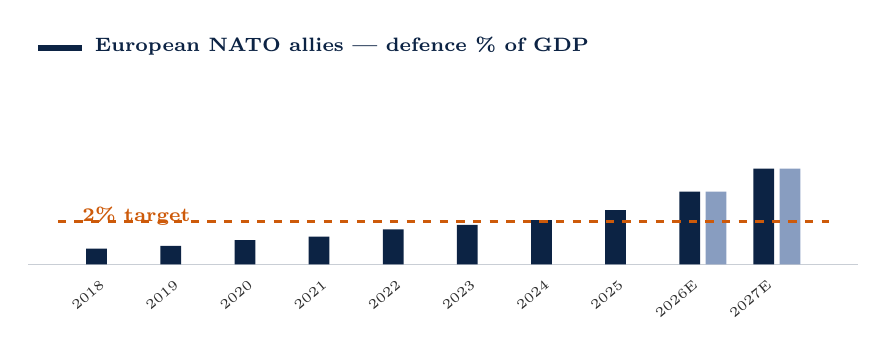
\begin{tikzpicture}
\begin{axis}[
  econ, height=3.85cm,
  ybar, bar width=7.5pt,
  title={\er European NATO allies — defence \% of GDP},
  ylabel={\% of GDP},
  ylabel style={at={(axis description cs:-0.05,0.5)},rotate=90},
  ytick={1.5,2.0,2.5,3.0,3.5},
  ymin=1.35, ymax=4.05,
  xtick={1,2,3,4,5,6,7,8,9,10},
  xticklabels={2018,2019,2020,2021,2022,2023,2024,2025,2026E,2027E},
  x tick label style={rotate=40,anchor=east,font=\tiny},
  xmin=0.5, xmax=10.5,
  enlarge x limits=0.06,
]
%% European Allies + Canada collective % GDP
%% Confirmed anchors from NATO official report (Aug 2025):
%%  2014 = 1.43%; 2024 = 2.02% (all European allies first time)
%%  2025 = all 32 allies >= 2% for first time (NATO summit Aug 2025 report)
%%  New Hague summit target: 3.5–5% by 2035
\addplot[fill=navy,draw=none] coordinates {
  (1,1.59)(2,1.63)(3,1.72)(4,1.77)
  (5,1.88)(6,1.95)(7,2.02)(8,2.17)
  (9,2.45)(10,2.80)
};
%% Projected bars lighter
\addplot[fill=navymid!55,draw=none] coordinates {
  (9,2.45)(10,2.80)
};
\draw[amber,thick,dashed]
  (axis cs:0.3,2.0) -- (axis cs:10.7,2.0);
\node[font=\scriptsize\bfseries,amber,anchor=west] at (axis cs:0.50,2.08)
  {2\% target};
\end{axis}
\end{tikzpicture}
\src{NATO Defence Expenditure of NATO Countries (2014–2025), Aug\,2025. 2018–2024 official; 2025–2027 NATO/analyst estimates. 2024\,=\,2.02\% confirmed (first time).}
\end{column}

\end{columns}
\end{frame}

%%% ═══════════════════════════════════════════════════════════════════════════
%%% 06 · HORIZON LENS
%%% ═══════════════════════════════════════════════════════════════════════════
\begin{frame}{06 · Investment Horizon Lens}

\begin{tikzpicture}[
  band/.style={rectangle,rounded corners=3pt,
               text width=3.52cm,minimum height=2.4cm,
               align=left,inner sep=8pt},
]
  \node[band,fill=navy](S) at (0,0) {%
    \color{white}\scriptsize\textbf{Short · Now → 1 yr}\\[4pt]
    \color{ice!90}\tiny
    Liquidity \& safe havens dominate\\[2pt]
    · USD, short Treasuries, gold\\
    · High-grade credit\\
    · Avoid illiquid frontier assets};

  \node[band,fill=navymid](M) at (4.0,0) {%
    \color{white}\scriptsize\textbf{Medium · 1 → 5 yrs}\\[4pt]
    \color{ice!90}\tiny
    Project finance converts into capex\\[2pt]
    · Ports, rail, defense supply chains\\
    · Mining project-finance closes\\
    · Infrastructure commitments};

  \node[band,fill=navy!65](L) at (8.0,0) {%
    \color{white}\scriptsize\textbf{Long · 5+ yrs}\\[4pt]
    \color{ice!90}\tiny
    Regional ecosystems emerge\\[2pt]
    · Mineral refining corridors\\
    · SMR fleet deployment\\
    · Sovereign digital infrastructure};

  \draw[->,thick,steel!60](S.east)--(M.west);
  \draw[->,thick,steel!60](M.east)--(L.west);

  %% timeline bar
  \draw[steel!40,line width=4pt]
    ([yshift=-1.1cm]S.south west) -- ([yshift=-1.1cm]L.south east);
  \foreach \xoff/\lbl in {0/2026, 2.67/2027, 5.33/2029, 8.0/2031+}{%
    \draw[navy,thin]
      ([xshift=\xoff cm,yshift=-0.90cm]S.south west) --
      ([xshift=\xoff cm,yshift=-1.30cm]S.south west);
    \node[font=\tiny,coal]
      at ([xshift=\xoff cm,yshift=-1.58cm]S.south west) {\lbl};
  }
\end{tikzpicture}

\vspace{8pt}
\begin{block}{\small Key principle}
  {\footnotesize
    Commitment events — not headlines — mark the shift from
    intent to deployed capital.}
\end{block}
\end{frame}

%%% ═══════════════════════════════════════════════════════════════════════════
%%% 07 · INSTRUMENTS
%%% ═══════════════════════════════════════════════════════════════════════════
\begin{frame}{07 · Instrument Suggestions — Example ETFs}
\begin{columns}[T,totalwidth=\textwidth]

\begin{column}{0.57\textwidth}
\renewcommand{\arraystretch}{1.28}
\setlength{\tabcolsep}{3pt}
\begin{tabular}{>{\scriptsize\bfseries}p{1.8cm}%
                >{\scriptsize\ttfamily}p{1.2cm}%
                >{\scriptsize}p{2.0cm}%
                >{\scriptsize}p{1.5cm}}
  \rowcolor{navy}
    \color{white}Allocation & \color{white}Ticker & \color{white}Name & \color{white}Theme \\
  \rowcolor{ice}
    Core\ 60–70\% & ACWI & iShares MSCI ACWI & Global baseline \\
  Defense A & XAR & SPDR Aero \& Defense & US primes \\
  \rowcolor{ice}
    Defense B & EUAD & VanEck Defense & European primes \\
  Cyber & CIBR & First Trust Cyber & Digital sovereignty \\
  \rowcolor{ice}
    Resources & REMX & VanEck Rare Earth & Minerals/battery \\
  Infrastructure & IGF & iShares Global Infra & Ports + corridors \\
\end{tabular}
\vspace{4pt}
{\tiny\color{coal}
  Not investment advice. ETF examples for educational framing only.
  Verify fees, AUM, liquidity and domicile before investing.}
\end{column}

\begin{column}{0.43\textwidth}
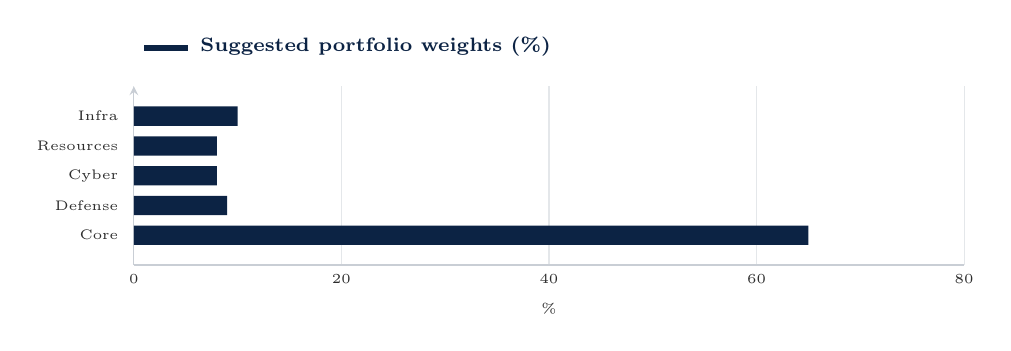
\begin{tikzpicture}
\begin{axis}[
  econh, height=3.85cm,
  title={\er Suggested portfolio weights (\%)},
  xlabel={\%},
  xlabel style={font=\tiny},
  ytick={1,2,3,4,5},
  yticklabels={Core,Defense,Cyber,Resources,Infra},
  xmin=0, xmax=80,
  xtick={0,20,40,60,80},
]
\addplot[fill=navy,draw=none] coordinates {
  (65,1)(9,2)(8,3)(8,4)(10,5)
};
\end{axis}
\end{tikzpicture}
\src{Example weights — not investment advice. Adjust to risk tolerance.}
\end{column}

\end{columns}
\end{frame}

%%% ═══════════════════════════════════════════════════════════════════════════
%%% 08 · WEEKLY WATCHLIST
%%% ═══════════════════════════════════════════════════════════════════════════
\begin{frame}{08 · Weekly Watchlist \& Triggers}

\begin{tikzpicture}[
  box/.style={rectangle,rounded corners=2pt,fill=ice,
              inner sep=6pt,text width=2.82cm,
              minimum height=2.25cm,align=left},
]
  \node[box](A) at (0,0) {%
    \textcolor{navy}{\small\bfseries Commitment Events}\\[4pt]
    \tiny · Offtake agreements\\
    · Project-finance close\\
    · Construction starts\\
    · Sovereign guarantees};

  \node[box](B) at (3.15,0) {%
    \textcolor{navy}{\small\bfseries Policy \& Budgets}\\[4pt]
    \tiny · Defense budgets (\%GDP)\\
    · Domestic content rules\\
    · Export controls\\
    · Procurement tenders};

  \node[box](C) at (6.30,0) {%
    \textcolor{navy}{\small\bfseries Market Evidence}\\[4pt]
    \tiny · FDI inflow data\\
    · M\&A / consolidation\\
    · DFI co-financing\\
    · Order backlog trends};

  \node[box](D) at (9.45,0) {%
    \textcolor{navy}{\small\bfseries Macro Triggers}\\[4pt]
    \tiny · DXY (dollar index)\\
    · 3-month Treasury yield\\
    · Shipping advisories\\
    · GPR index reading};

  \foreach \n in {A,B,C,D}{%
    \draw[navy,line width=2pt]
      (\n.north west) -- (\n.north east);}
\end{tikzpicture}

\vspace{8pt}
{\small\color{coal}
  Check \textbf{all four panels} weekly.
  Headline noise without commitment-event confirmation
  = signal to filter, not act on.}
\end{frame}

%%% ═══════════════════════════════════════════════════════════════════════════
%%% 09 · WARNINGS
%%% ═══════════════════════════════════════════════════════════════════════════
\begin{frame}{09 · Warnings \& Guardrails}
\begin{columns}[T,totalwidth=\textwidth]

\begin{column}{0.54\textwidth}
\renewcommand{\arraystretch}{1.34}
\begin{tabular}{>{\scriptsize\bfseries\color{navy}}p{2.55cm}%
                >{\footnotesize}p{3.85cm}}
  \toprule
  Risk & What it means \\
  \midrule
  Timing risk &
    Headlines create volatility; commitment events matter more \\
  Valuation risk &
    Thematic ETFs can spike sharply after headline rallies \\
  Liquidity risk &
    Frontier/thematic exposures can be illiquid \\
  FX \& sovereign risk &
    EM corridors carry FX + political risk \\
  Sanctions risk &
    Defense \& dual-use chains face export-control risk \\
  \bottomrule
\end{tabular}
\end{column}

\begin{column}{0.44\textwidth}
\begin{block}{Simple mitigation framework}
  {\footnotesize
  \begin{itemize}
    \item \textbf{Core first}: 60–70\% in broad market ETF
    \item \textbf{Small satellites}: 5–10\% per theme max
    \item \textbf{Weekly discipline}: watchlist, not news feed
    \item \textbf{Liquid vehicles}: ETF over single stock
    \item \textbf{No single-country bets}: diversify geography
  \end{itemize}}
\end{block}
\end{column}

\end{columns}
\end{frame}

%%% ═══════════════════════════════════════════════════════════════════════════
%%% 10 · WEEKLY CHECKS
%%% ═══════════════════════════════════════════════════════════════════════════
\begin{frame}{10 · Weekly Discipline — Checklist}
\begin{columns}[T,totalwidth=\textwidth]

\begin{column}{0.47\textwidth}
{\scriptsize\bfseries\color{navy}Every week, check these six signals:}\\[6pt]
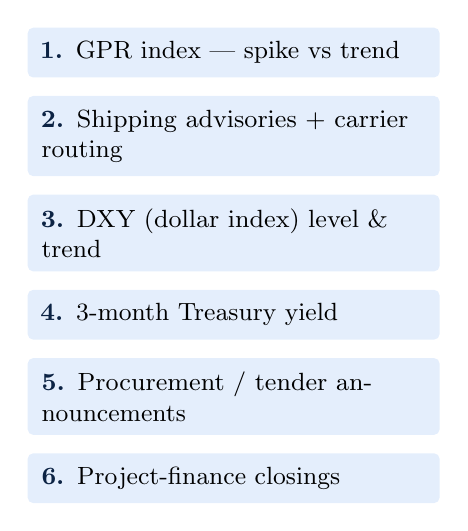
\begin{tikzpicture}[
  item/.style={rectangle,fill=ice,rounded corners=2pt,
               text width=4.88cm,inner sep=5pt,
               font=\small,align=left},
  node distance=0.22cm,
]
  \node[item](i1){\textbf{\color{navy}1.}\enspace GPR index — spike vs trend};
  \node[item,below=of i1](i2){\textbf{\color{navy}2.}\enspace Shipping advisories + carrier routing};
  \node[item,below=of i2](i3){\textbf{\color{navy}3.}\enspace DXY (dollar index) level \& trend};
  \node[item,below=of i3](i4){\textbf{\color{navy}4.}\enspace 3-month Treasury yield};
  \node[item,below=of i4](i5){\textbf{\color{navy}5.}\enspace Procurement / tender announcements};
  \node[item,below=of i5](i6){\textbf{\color{navy}6.}\enspace Project-finance closings};
\end{tikzpicture}
\end{column}

\begin{column}{0.51\textwidth}
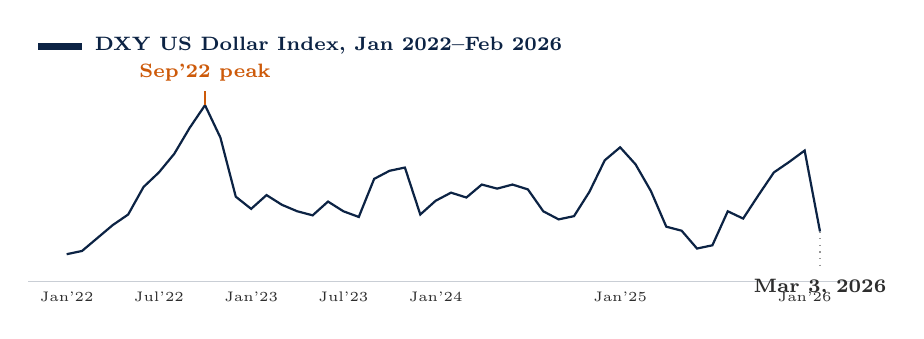
\begin{tikzpicture}
\begin{axis}[
  econ, height=4.05cm,
  title={\er DXY US Dollar Index, Jan 2022–Feb 2026},
  ylabel={Index},
  ylabel style={at={(axis description cs:-0.05,0.5)},rotate=90},
  ytick={96,100,104,108,112},
  ymin=93, ymax=117,
  xtick={1,7,13,19,25,37,49},
  xticklabels={Jan'22,Jul'22,Jan'23,Jul'23,Jan'24,Jan'25,Jan'26},
  xmin=0.5, xmax=50.5,
]
%% Monthly DXY close Jan 2022 – Feb 2026 (sequential month 1..50)
%% Confirmed anchors:
%%  Jan 2022 start ~96; Sep/Oct 2022 peak 114.78 (confirmed 20-yr high);
%%  End 2022: 103.52 (confirmed); Mar 2023: ~103.5;
%%  End 2023: ~101; End 2024: ~108 (DXY rose ~7% in 2024 H2);
%%  Mar 3 2026: 99.2 (confirmed live)
\addplot[navy,thick,mark=none] coordinates {
  % 2022 Jan–Dec: rate-hike surge to Sep peak then partial reversal
  (1, 96.4)(2, 96.8)(3, 98.4)(4,100.0)(5,101.3)(6,104.7)
  (7,106.5)(8,108.8)(9,112.0)(10,114.8)(11,110.8)(12,103.5)
  % 2023 Jan–Dec: gradual easing of dollar
  (13,102.0)(14,103.7)(15,102.5)(16,101.7)(17,101.2)(18,102.9)
  (19,101.7)(20,101.0)(21,105.7)(22,106.7)(23,107.1)(24,101.3)
  % 2024 Jan–Dec: initially soft, strong late-year rally on Trump election
  (25,103.0)(26,104.0)(27,103.4)(28,105.0)(29,104.5)(30,105.0)
  (31,104.4)(32,101.7)(33,100.7)(34,101.1)(35,104.1)(36,108.0)
  % 2025 Jan–Dec: tariff uncertainty, dollar volatile
  (37,109.6)(38,107.5)(39,104.2)(40,99.8)(41,99.3)(42,97.1)
  (43,97.5)(44,101.7)(45,100.8)(46,103.7)(47,106.5)(48,107.8)
  % 2026 Jan–Feb
  (49,109.2)(50, 99.2)
};
\draw[amber,thin]
  (axis cs:10,114.8) -- (axis cs:10,116.5)
  node[anchor=south,font=\scriptsize\bfseries,amber]{Sep'22 peak};
\draw[coal!50,thin,dotted]
  (axis cs:50,99.2) -- (axis cs:50,94.5)
  node[anchor=north,font=\scriptsize\bfseries,coal]{Mar 3, 2026};
\end{axis}
\end{tikzpicture}
\src{DXY (ICE / FRED). Sep\,2022 peak\,=\,114.78 confirmed; end-2022\,=\,103.5; Mar\,3\,2026\,=\,99.2 confirmed.}
{\tiny\color{coal}
  Rising DXY + elevated GPR = headwind for EM debt. Watch EM spreads.}
\end{column}

\end{columns}
\end{frame}

%%% ═══════════════════════════════════════════════════════════════════════════
%%% BRIEFING A — CRITICAL MINERALS
%%% ═══════════════════════════════════════════════════════════════════════════
\begin{frame}{Briefing A · Critical Minerals \& African Corridors}
\begin{columns}[T,totalwidth=\textwidth]

\begin{column}{0.50\textwidth}
{\scriptsize\bfseries\color{navy}What to watch}\\[4pt]
{\footnotesize\begin{itemize}\setlength\itemsep{3pt}
  \item \textbf{Offtake agreements} — volume, term, counterparty credit
  \item \textbf{Project-finance close} — lenders, guarantees, DFI co-funding
  \item \textbf{Corridor construction milestones} — schedule vs plan
  \item \textbf{Political signals} — expropriation risk, DRC/Zambia stability
  \item \textbf{Copper/cobalt spot + futures} — entry and sizing signals
\end{itemize}}
\vspace{6pt}
\begin{block}{\small Deploy capital when}
{\footnotesize Offtake \textit{and} project-finance close \textit{and} construction
start are all confirmed simultaneously.}
\end{block}
\end{column}

\begin{column}{0.48\textwidth}
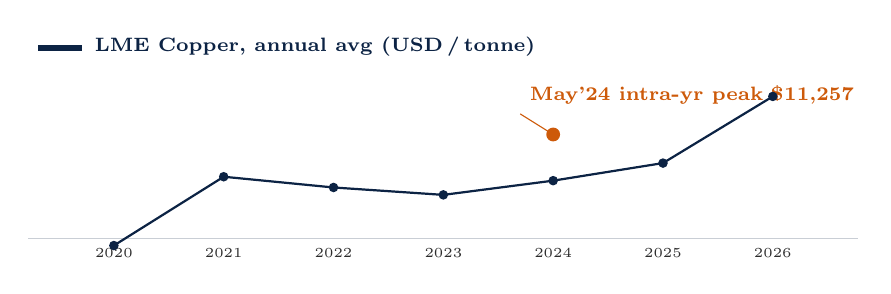
\begin{tikzpicture}
\begin{axis}[
  econ, height=3.55cm,
  title={\er LME Copper, annual avg (USD\,/\,tonne)},
  ylabel={USD/t},
  ylabel style={at={(axis description cs:-0.05,0.5)},rotate=90},
  ytick={7000,8000,9000,10000,11000,12000},
  ymin=6500, ymax=13600,
  xtick={1,2,3,4,5,6,7},
  xticklabels={2020,2021,2022,2023,2024,2025,2026},
  xmin=0.5, xmax=7.5,
]
%% Annual average LME copper price USD/tonne
%% Confirmed anchors (FRED IMF annual series PCOPPUSDA):
%%  2023 = $8,491; 2024 = $9,142; 2025 = $9,947 (annual avg)
%%  May 2024 intra-year peak: ~$11,257 (Comex, confirmed record)
%%  Jan 2026 monthly: ~$12,987 (FRED PCOPPUSDM confirmed)
%%  Mar 2, 2026 spot: $13,230 (KME confirmed)
\addplot[navy,thick,mark=*,mark options={fill=navy,scale=0.65}] coordinates {
  (1,6170)(2,9322)(3,8830)(4,8491)(5,9142)(6,9947)(7,13000)
};
%% Note peak annotation
\draw[amber,thin]
  (axis cs:5,11257) -- (axis cs:4.7,12200)
  node[anchor=south west,font=\scriptsize\bfseries,amber]{May'24 intra-yr peak \$11{,}257};
%% Peak dot
\fill[amber] (axis cs:5,11257) circle (2.5pt);
\end{axis}
\end{tikzpicture}
\src{LME/IMF via FRED (PCOPPUSDM/A). 2021 avg\,=\,\$9{,}322; 2023\,=\,\$8{,}491; 2024\,=\,\$9{,}142; 2025\,=\,\$9{,}947 confirmed. Jan\,2026\,=\,\$12{,}987; spot Mar\,3\,2026\,=\,\$13{,}230.}
\end{column}

\end{columns}
\end{frame}

%%% ═══════════════════════════════════════════════════════════════════════════
%%% BRIEFING B — DEFENSE
%%% ═══════════════════════════════════════════════════════════════════════════
\begin{frame}{Briefing B · Defense \& Dual-use Manufacturing}
\begin{columns}[T,totalwidth=\textwidth]

\begin{column}{0.50\textwidth}
{\scriptsize\bfseries\color{navy}What to watch}\\[4pt]
{\footnotesize\begin{itemize}\setlength\itemsep{3pt}
  \item \textbf{Budget laws} — multi-year commitments (\% GDP + EUR totals)
  \item \textbf{Procurement awards} — contract value, timeline, local-content clauses
  \item \textbf{Order-backlog growth} — prime contractor quarterly reports
  \item \textbf{Export-control shifts} — component supply-chain disruptions
\end{itemize}}
\vspace{6pt}
\begin{block}{\small Deploy when}
{\footnotesize Budget law enacted \textit{and} procurement tender awarded
\textit{and} order-backlog growth confirmed in quarterly results.}
\end{block}
\end{column}

\begin{column}{0.48\textwidth}
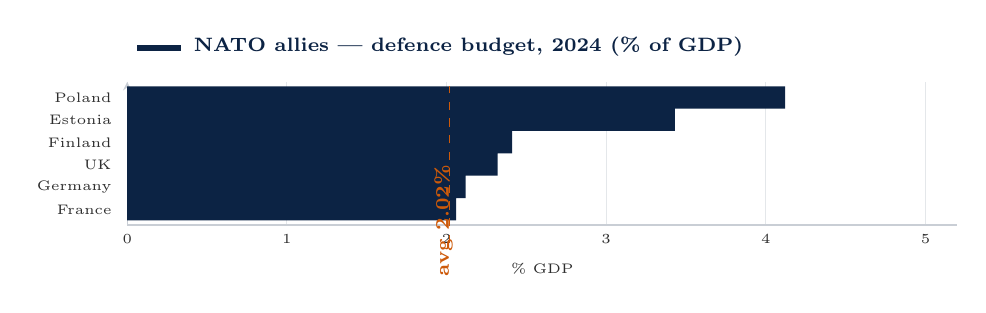
\begin{tikzpicture}
\begin{axis}[
  econh, height=3.4cm,
  title={\er NATO allies — defence budget, 2024 (\% of GDP)},
  xlabel={\% GDP},
  xlabel style={font=\tiny},
  ytick={1,2,3,4,5,6},
  yticklabels={France,Germany,UK,Finland,Estonia,Poland},
  xmin=0, xmax=5.2,
  xtick={0,1,2,3,4,5},
  bar width=8pt,
  enlarge y limits=0.14,
]
%% Official NATO data (NATO Defence Expenditure report, Aug 2025)
%% European NATO average 2024 = 2.02% (confirmed)
%% Country estimates: Poland 4.12% (confirmed highest); Estonia ~3.43%;
%% Finland ~2.41%; UK ~2.32%; Germany ~2.12%; France ~2.06%
\addplot[fill=navy,draw=none] coordinates {
  (2.06,1)(2.12,2)(2.32,3)(2.41,4)(3.43,5)(4.12,6)
};
\draw[amber,thin,dashed]
  (axis cs:2.02,-0.5) -- (axis cs:2.02,6.5);
\node[font=\scriptsize\bfseries,amber,rotate=90,anchor=south] at (axis cs:2.10,0.5)
  {avg 2.02\%};
\end{axis}
\end{tikzpicture}
\src{NATO Defence Expenditure of NATO Countries (2014–2025), Aug\,2025.
European NATO average 2024\,=\,2.02\% (confirmed first time).}
\end{column}

\end{columns}
\end{frame}

%%% ═══════════════════════════════════════════════════════════════════════════
%%% BRIEFING C — ASEAN
%%% ═══════════════════════════════════════════════════════════════════════════
\begin{frame}{Briefing C · ASEAN Manufacturing — Vietnam Hub}
\begin{columns}[T,totalwidth=\textwidth]

\begin{column}{0.50\textwidth}
{\scriptsize\bfseries\color{navy}What to watch}\\[4pt]
{\footnotesize\begin{itemize}\setlength\itemsep{3pt}
  \item \textbf{FDI disbursed} — monthly official data (Vietnam MPI)
  \item \textbf{Factory construction starts} — industrial-park activity
  \item \textbf{Electronics export growth} — monthly trade data
  \item \textbf{Tariff and trade policy} — shifts affecting relocation decisions
\end{itemize}}
\vspace{6pt}
\begin{block}{\small Deploy when}
{\footnotesize FDI disbursements rising \textit{and} factory construction started
\textit{and} export diversification confirmed in monthly trade data.}
\end{block}
\end{column}

\begin{column}{0.48\textwidth}
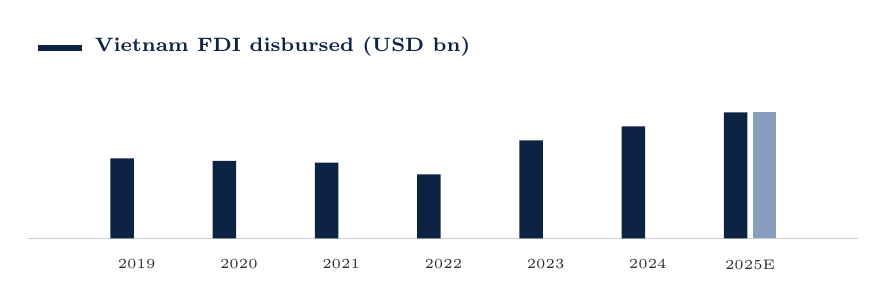
\begin{tikzpicture}
\begin{axis}[
  econ, height=3.55cm,
  ybar, bar width=8.5pt,
  title={\er Vietnam FDI disbursed (USD bn)},
  ylabel={USD bn},
  ylabel style={at={(axis description cs:-0.05,0.5)},rotate=90},
  ytick={10,15,20,25,30},
  ymin=8, ymax=32,
  xtick={1,2,3,4,5,6,7},
  xticklabels={2019,2020,2021,2022,2023,2024,2025E},
  xmin=0.5, xmax=7.5,
  enlarge x limits=0.08,
]
%% Vietnam FDI Disbursed (realized) USD billions — OFFICIAL DATA
%% Confirmed anchors (VietnamPlus / MPI official):
%%  2022: 17.90 bn (confirmed World Bank); 2023: 23.18 bn (confirmed, +3.5% vs 2022);
%%  2024: 25.35 bn (confirmed, record high, +9.4% vs 2023)
%%  2019: 20.38 bn; 2020: 19.98 bn; 2021: 19.74 bn (VietnamPlus)
\addplot[fill=navy,draw=none] coordinates {
  (1,20.38)(2,19.98)(3,19.74)(4,17.90)(5,23.18)(6,25.35)(7,27.5)
};
%% 2025E bar lighter
\addplot[fill=navymid!55,draw=none] coordinates {
  (7,27.5)
};
\end{axis}
\end{tikzpicture}
\src{Vietnam MPI / VietnamPlus. 2022\,=\,\$17.9\,bn; 2023\,=\,\$23.2\,bn; 2024\,=\,\$25.35\,bn (record high, +9.4\% y/y) — confirmed official data.}
\end{column}

\end{columns}
\end{frame}

%%% ═══════════════════════════════════════════════════════════════════════════
%%% BRIEFING D — LOBITO CORRIDOR SPOTLIGHT
%%% ═══════════════════════════════════════════════════════════════════════════
\begin{frame}{Briefing D · Lobito Corridor — Critical Minerals, \$6 bn+ Committed}
\begin{columns}[T,totalwidth=\textwidth]

\begin{column}{0.50\textwidth}
{\scriptsize\bfseries\color{navy}\er What it is}\\[2pt]
{\footnotesize\color{coal}
  Lobito port (Angola) → DRC copper belt → Zambia.
  800\,km existing rail + 1,300\,km extension.
  The spine of global copper and cobalt supply.}

\vspace{3pt}
{\scriptsize\bfseries\color{navy}\er Capital committed (Dec 2025)}\\[2pt]
\renewcommand{\arraystretch}{1.18}
\setlength{\tabcolsep}{3pt}
{\footnotesize
\begin{tabular}{>{\bfseries\color{navy}}p{2.0cm}>{\footnotesize}p{3.0cm}}
  \rowcolor{ice} \$535\,M (Dec'25) & DFC + Trafigura + Mota-Engil \\
  Total committed & \textbf{\$6\,bn+} (US, EU, AfDB, private) \\
  \rowcolor{ice} DRC–US deal & Strategic minerals access \\
  EU & €200\,M Zambia energy/mining \\
\end{tabular}}

\vspace{3pt}
{\scriptsize\bfseries\color{navy}\er Why copper matters now}\\[2pt]
{\footnotesize\color{coal}
  EV: 83\,kg Cu each. Offshore wind turbine: 4–15\,t.
  Copper at \$13{,}230/t (Mar 3, 2026) — up 56\% vs 2023.}
\end{column}

\begin{column}{0.48\textwidth}
%% Timeline of key commitment events
{\scriptsize\bfseries\color{navy}\er Commitment event timeline}\\[3pt]
\begin{tikzpicture}[
  ev/.style={rectangle,rounded corners=1pt,fill=ice,
             inner sep=3pt,text width=5.2cm,align=left,font=\tiny},
  dt/.style={font=\tiny\bfseries,color=navy,anchor=west},
]
  \draw[navy!30,line width=1.5pt] (0.9,0.1) -- (0.9,-4.7);
  \node[dt] at (0.0, -0.0) {2023};
  \node[ev,anchor=west] at (1.1,-0.0) {G7 endorses corridor; EU commits to Partnership for Global Infrastructure};
  \node[dt] at (0.0,-1.0) {Mar'24};
  \node[ev,anchor=west] at (1.1,-1.0) {AfDB \$200\,M + US DFC \$250\,M first tranche. Construction mobilises};
  \node[dt] at (0.0,-2.0) {Jun'24};
  \node[ev,anchor=west] at (1.1,-2.0) {EU €300\,M Global Gateway; Trafigura offtake agreement signed};
  \node[dt] at (0.0,-3.0) {Dec'25};
  \node[ev,anchor=west,fill=navy!15] at (1.1,-3.0) {\textbf{DFC+Trafigura \$535\,M closes.} US–DRC strategic mineral access deal signed};
  \node[dt] at (0.0,-4.0) {Mar'26};
  \node[ev,anchor=west,fill=amber!20] at (1.1,-4.0) {Cu \$13{,}230/t — total committed \textbf{>\,\$6\,bn} — construction active};
\end{tikzpicture}
\src{US DFC, AfDB, EU Commission press releases. Copper: LME / KME Mar 3, 2026.}
\end{column}

\end{columns}
\end{frame}

\end{document}
